\section{Negative results}
\label{app:negative}
\begin{figure}
  \centering
  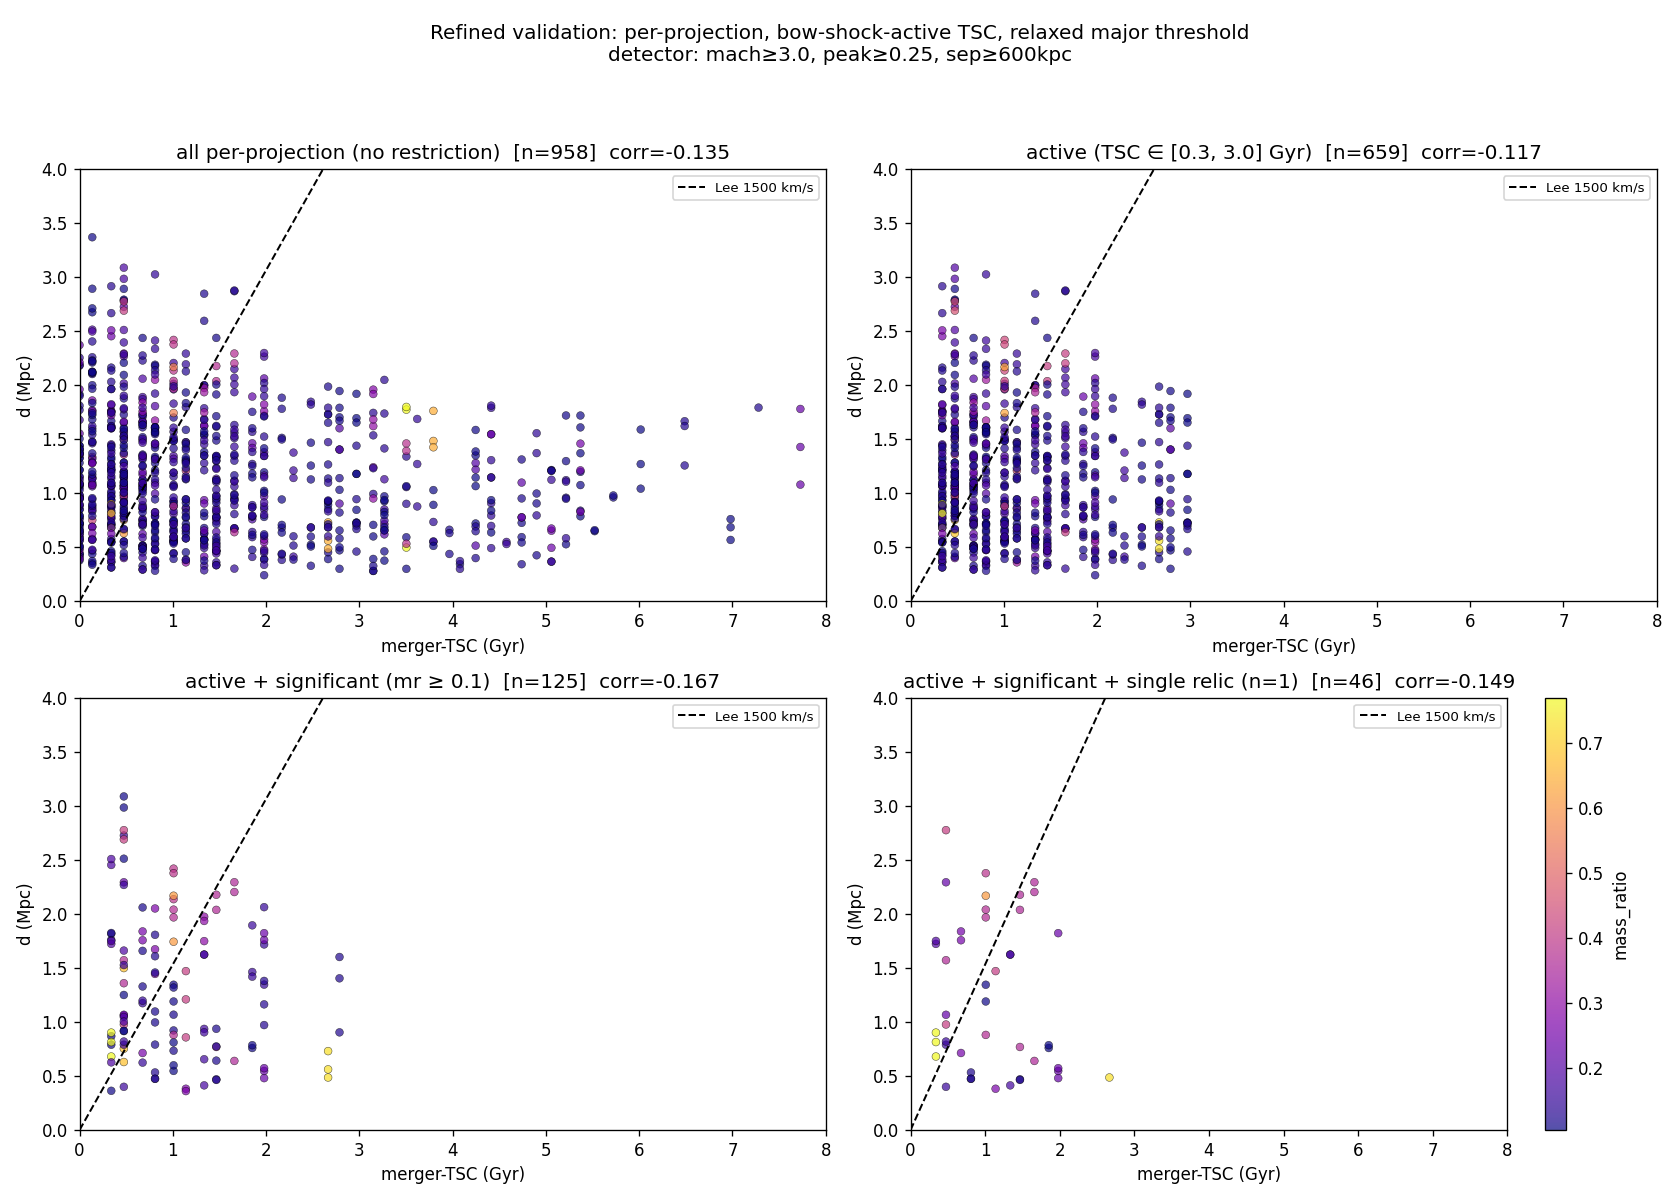
\includegraphics[width=\columnwidth]{relic_v3_validation.png}
  \caption{Relic separation against merger time in TNG-Cluster, four
  slicings: no positive relation.
  \stale{labels and centring predate the audit; re-check before use.}}
  \label{fig:relic_null}
\end{figure}

\begin{figure}
  \centering
  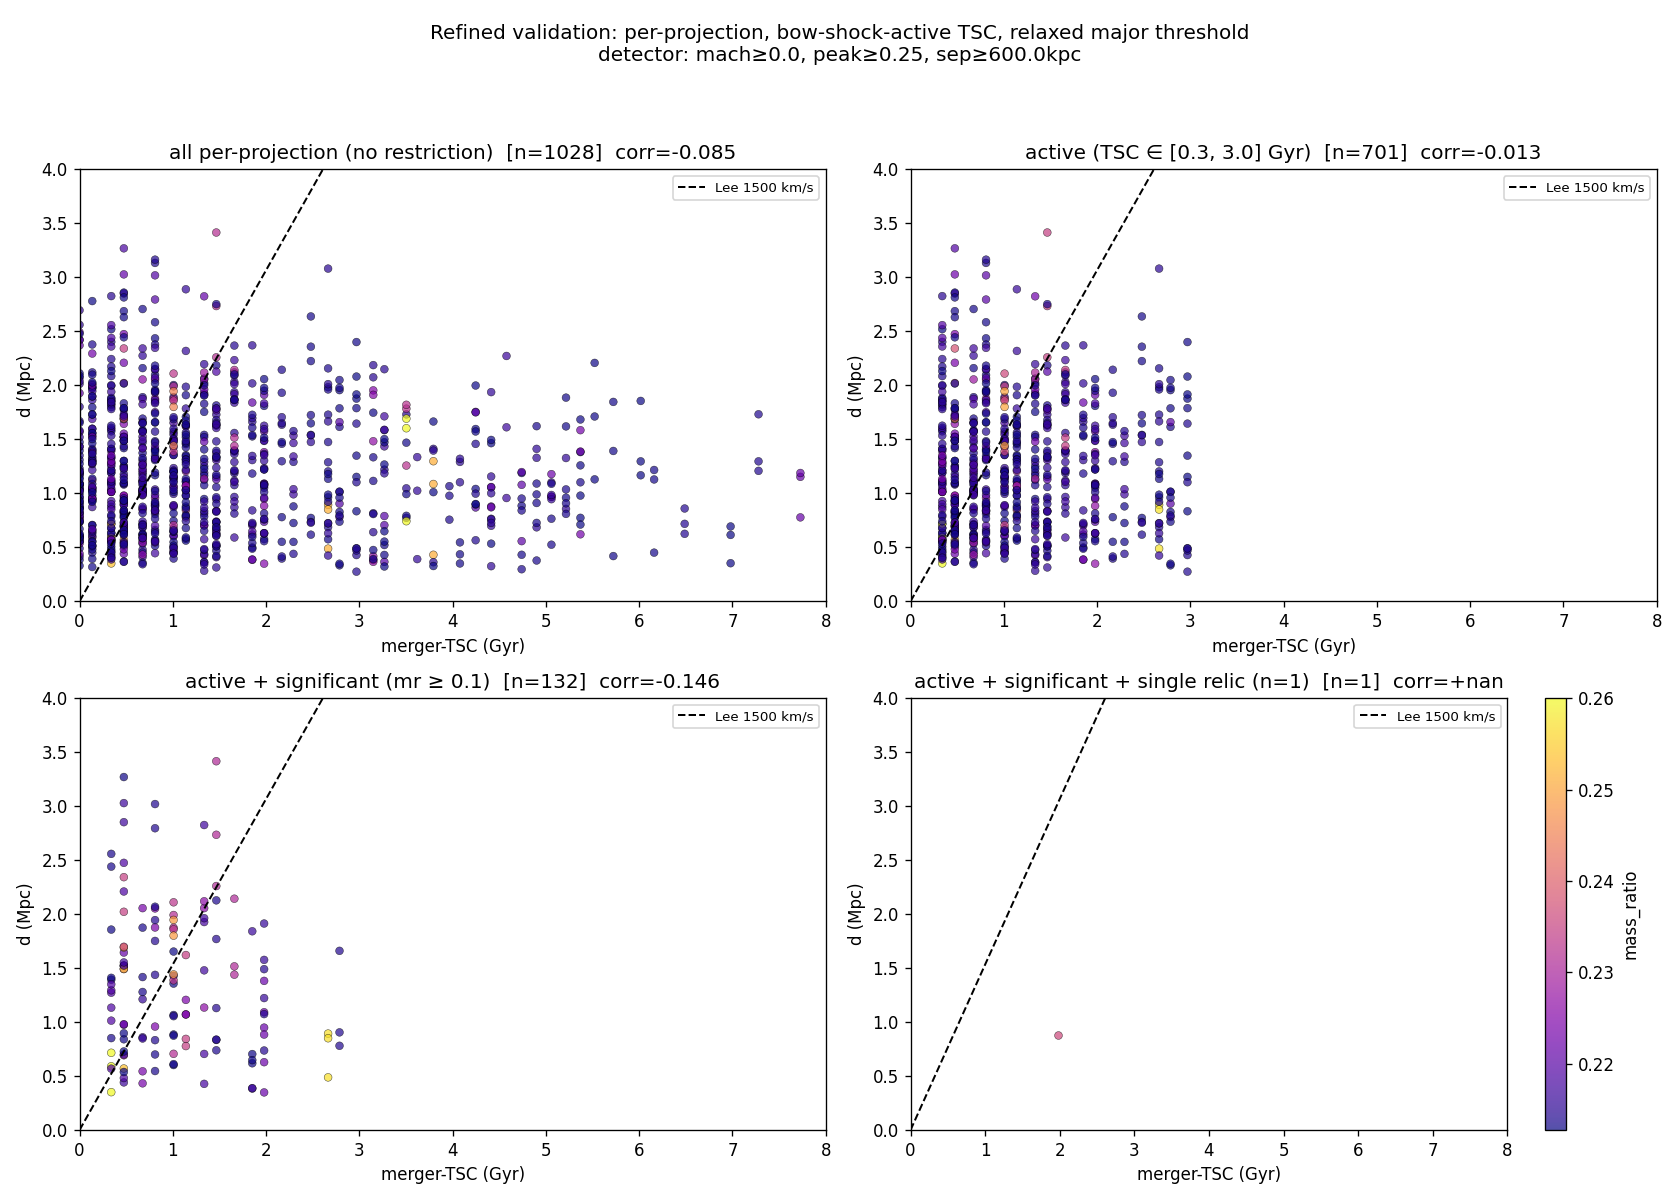
\includegraphics[width=\columnwidth]{relic_radio_validation.png}
  \caption{The same test with relics detected directly in the radio maps
  rather than from shock cells.
  \stale{predates the audit.}}
  \label{fig:relic_radio}
\end{figure}

\begin{figure}
  \centering
  \includegraphics[width=\columnwidth]{aug_comparison_128.png}
  \caption{CNN with and without diffusion-generated augmentation: no gain
  under cross-validation.
  \stale{single-split protocol shown; the 5-fold result (no gain,
  $\Delta R^2 = +0.001$) needs its own plot.}}
  \label{fig:aug}
\end{figure}

\begin{figure}
  \centering
  \includegraphics[width=\columnwidth]{camels_mass_tsc.png}
  \caption{CAMELS zooms: mass against the proxy merger time. Adding CAMELS
  to training did not help, because the label, not the images, is the
  bottleneck.}
  \label{fig:camels}
\end{figure}
